\chapter{Kommunikation}\label{ch:communication}
Som nævnt i sektion \ref{sec:distSys} foregår kommunikationen i flere lag, herunder frontend (præsentationslag), logik lag som tilgåes gennem QWest.API, og et datalag som er databasen, der tilgåes af QWest.DataAccess. 
Når programmet startes de forskellige services nævnt i sektion \ref{sec:servicesArc}. QWest.Web oprettes som en proxy der sender HTTP forespørgsler, og hele opstartsprocessen kan ses på figur \ref{fig:startup_log}.

\begin{figure}
    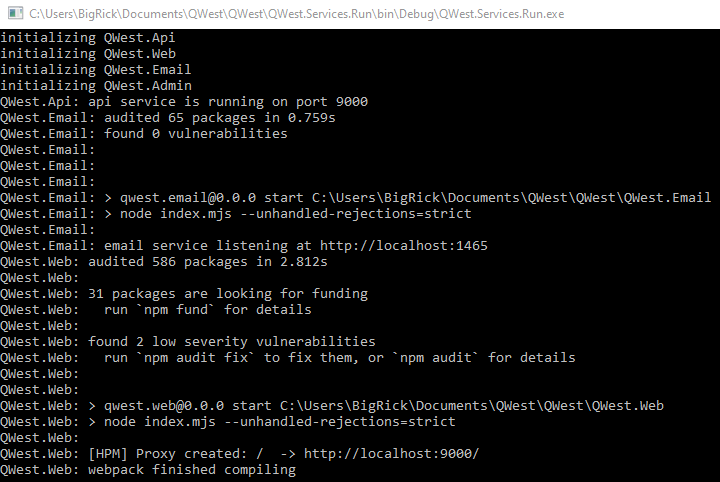
\includegraphics[width=\linewidth]{services_run_log.png}
    \caption{QWest.Services.Run opstarts log.}
    \label{fig:startup_log}
\end{figure}

Bruger-klienten tilgås gennem en browser, som sender HTTP-requests til QWest.API, der så kalder controllers til DAO til databasen. Som nævnt i sektion \ref{sec:REST} bruges der Json.NET til serialisering og JSON data til deserialisering. Da projektet er gennemført med REST, er der ingen konstant forbindelse til databasen, men i stedet laves der kun forbindelser når databasen skal opdateres ud fra en brugeroperation. 

\section{Sikkerhed}\label{sec:security}
HTTPS vil være den primærer måde at sikre os at bruger input er sikkert enkrypteret mens de bliver transporeret til QWest.Api, .NET framework skulle have support for HTTPS. \cite{DotNetFrameworkSSL} dog har der ikke været arbejde til at sætte dette op eftersom at vi ikke ejer it SSL certificate.
Måden autentificering er implementeret i systemet, er gennem login siden. Man skal være logget ind som bruger med brugernavn og password for at kunne tilgå andre dele af systemet. Hver file-path som kan tilgås på hjemmesiden, checker om det er den korrekte bruger der er logget ind. Hvis ikke, så sendes brugeren til forsiden hvor de kan logge ind eller oprette bruger.
For at sikre vores brugere mod leaking af deres passwords, hvis der sker et data breach, hasher og salter vi alle brugeres passwords. Der bruges \texttt{Rfc2898DeriveBytes} \cite{Rfc2898DeriveBytes} til dette. Denne klasse bruger SHA1, som er ikke er en optimal sikker hashing metode, hvilket burde ændres i næste iteration af projektet \cite{HowsecureisSHA1} til BCrypt \cite{BCrypt} eller lignende.
Når data skal lægges i databasen, bruges der SQL parametre for at undgå SQL injections. Som det kan ses i kodestykket \ref{lst:SQLinjection}, så bruges der en parametriseret SQL query string, hvor argumenterne metoden får placeres i de tilsvarende SQL parametre.

\begin{listing}[p]
    \begin{minted}
    [
        frame=lines,
        framesep=2mm,
        baselinestretch=1.2,
        bgcolor=LightGray,
        fontsize=\footnotesize,
        linenos,
        breaklines
    ]{csharp}
public async Task Update(Post post) {
    if (post.Id == null) {
        throw new ArgumentException("Editing a post needs a post ID");
    }
    string query = @"
UPDATE posts
SET content = @content
WHERE id = @post_id";
    await _conn.Use(query, async stmt => {
        stmt.Parameters.AddWithValue("@content", post.Contents);
        stmt.Parameters.AddWithValue("@post_id", post.Id);
        await stmt.ExecuteNonQueryAsync();
        return true;
    });
}
\end{minted}
\caption{QWest.DataAccess.Mssql.PostImpl\label{lst:SQLinjection}}
\end{listing}

\section{Transactions}\label{sec:transactions}
% Transactions
% Identify places in the application where we need transactions
% How do we build our transactions? Isolation levels?
% Do we need distributed transactions?
% ACID, Parallelism, Async/Await,
% Implementation details welcome
% Transactions and distributed systems from \cite{DistributedSystems}

\section{Protokoller}\label{sec:protocols}
Kommunikationen mellem alle services'ne i QWest er http requests, med untagelse af kommunikationen med databasen fra QWest.DataAccess. kommunikationen fra vores frontend web klient til QWest.Api (endten direkte eller proxiet gennem QWest.Web) skal selfølgelig være http eftersom at der ikke er webstandarder for andre muligheder, den eneste untagelse værende WebSockets, dog er dette ikke usecasen for WebSockets og WebSockets har ikke lige så stor support blandt ældrere browsere som en help normal http request har. Denne kommunikationen bruger igen JSON eftersom at frontend browser javascript ikke supporter mange andre måder at serializere og deserializere data på

Der kan argumenteres for brug af en anden type kommunikationen til og fra QWest.Email eftersom at node.js har muligheden for rå TCP og UDP, og en serializerings metode some protobuf \cite{ProtoBuf} eller binary serializering \cite{CsharpBinarySerialization} ville dette unødvendig kompleksitet ind i projektet og introdusere tredjepartsbiblioteker i enten QWest.Email eller andre services som bruger QWest.Email, derfor ender QWest.Email med at følge standarden sat af QWest.Api og bruge standard http requests der sender JSON serializeret data.

\section{Caching and HTTP optimization}\label{sec:caching}
Caching the concept of saving the result of an expensive operation and instead of doing the operation again, the cache is just returned instead. Denne pattern har fordellen at reducerer mængden af komputationer der skal laves, dog kan den kun implementeres steder hvor at data'en ikke behøver at opdateres ofte eller hvor at du ved resultatet af operationen vil alted være den samme. Et eksempel på det første kriterie kunne være en informationsskærm som fortæller gæster hvordan været af, koden bag denne behøver ikke at konstant spørge DMI's API efter hvordan været er, at spørge vær time er nok godt nok. Et eksempel på det andet kriterie kunne være vores QWest.Web service som serverer statiske filer, der er ingen grund til at læse fra filsystemet vær eneste gang der bliver lavet en request hvis fil'en allerede er i hukommelsen.

HTTP protokollen har også indbygget caching \cite{HTTPcaching}, oftest form af \texttt{Cache-Control header}'en der lader webserver fortælle browsere hvor land tid de cache resultated for denne specifikke url. I QWest bruges HTTP caching i vores REST API i QWest.Api når billeder bliver leveret, eftersom at vi ikke lader billeder ændre sig betyder det at flere end en HTTP request til \texttt{/api/Image/Get/<image\_id>} er overflødig, og vi kan derfor tælle browseren til at gemme resultatet (i dette tilfælge billedet) til næste gang billedet skal bruges. Cache tiden er nuværende sat til 8765 timer (ca. at år), eftersom at "immutable" ikke er implementeret i alle browserer endnu.

\section{Middleware}\label{sec:middleware}
QWest.Web bruger Owin \cite{Owin} til at leverer vores middleware. Det eneste stykke middleware skrevet manuelt er \texttt{QWest.Api.AuthenticationMiddleware} klassen, middleware'en checker om der er en authentikations token med i requestsen og hvis der er, hender den brugen som den token referer til og lægger den i OwinContext'en. 